\section{Ogólny zarys funkcjonowania programu}
Autorski program, mający na celu przetworzenie danych ze skanera 3D w celu uzyskania modeli trójwymiarowych składa się z wielu istotnych kroków. Począwszy od wczytania danych z kamery trójwymiarowej, a skończywszy na eksportowaniu modeli do programu Blender. Istnieje wiele różnych podejść do implementacji poniższych algorytmów. Poniżej zostaną omówione autorskie metody na ich implementację oraz optymalizację. W rozdziale zostaną opisane najważniejsze algorytmy oraz ich szczegółowe charakterystyki. Program zawiera graficzny interfejs, który ma umożliwić użytkownikom łatwą obróbkę danych.
\subsection{Odczytanie danych z kamery RGBD}
Pierwszym krokiem pracy programu jest odczytanie danych z kamery trójwymiarowej. Wczytane dane są poddawane różnym obróbkom w celu usunięcia przekłamań spowodowanych złymi odczytami z czujnika głębi. Głównym tego powodem jest rozpraszanie wiązki światła na obiekcie, co uniemożliwia poprawny odczyt głębi przez skaner. Przykład takiej sytuacji został przedstawiony na rysunku \ref{fig:depthErrorImage}.
\begin{figure}[H]
  \centering
  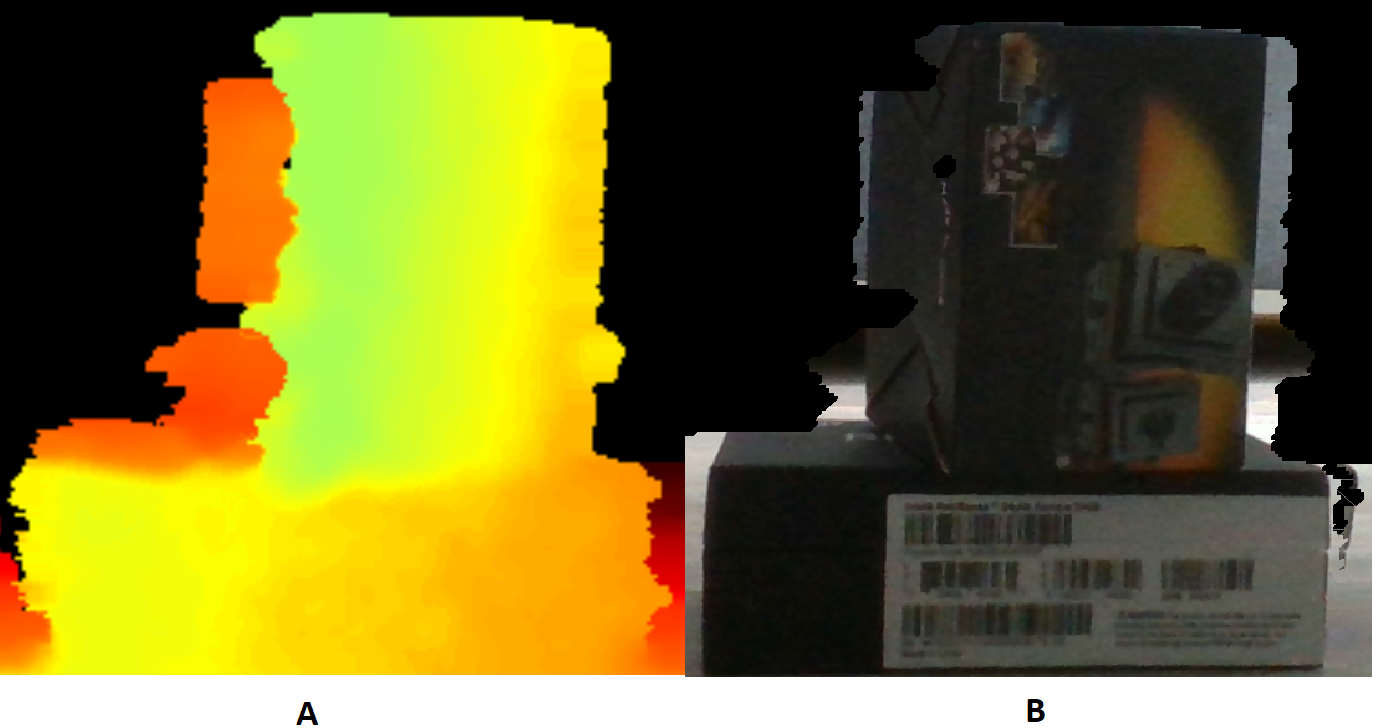
\includegraphics[scale=0.4]{pudelko_glebia_kolor.png}
  \caption{A-Zniekształcona głębia, B-Głębia z nałożoną teksturą RGB}   
  \label{fig:depthErrorImage}
\end{figure}
Biblioteka PyRealSense dostarczana przez firmę Intel do kamer trójwymiarowych zapewnia szereg funkcji pozwalających na oczyszczenie wynikowych danych z dziur. W pakiecie SDK zawarte są filtry chwilowe oraz przestrzenne. Filtr chwilowy umożliwia wypełnienie dziur wartościami z poprzednich klatek. Jest to funkcja, która pozwala na uzyskanie bardziej czytelnych danych. Są one również wiarygodniejsze niż użycie interpolacji do uzyskania danych. Filtr przestrzenny umożliwia wygładzenie danych zachowując jednocześnie dane brzegowe. W przypadku wcześniejszego filtru te dane są tracone w skutek mieszania danych z aktualnych oraz wcześniejszych klatek. Przydatna okazuje się również być funkcja do nakładania na siebie obrazu głębi oraz koloru. Czujnik natężenia siatki światła oraz kamera RGB znajdują się obok siebie, dlatego też piksel o współrzędnych (x,y) będzie różnił się w przypadku koloru oraz głębi \cite{IntelRealSenseSheet}. By uzyskać poprawne dane trzeba nałożyć odpowiednio klatki pochodzące z kamery RGB oraz czujnika głębi. Zostało to dokonane poprzez wykorzystanie odpowiedniej funkcji z biblioteki PyRealSense. Możliwy jest wybór względem, którego źródła mają być nakładane na siebie klatki. Na potrzeby programu klatki nakładane są na siebie względem ujęcia RGB.

Następnym krokiem jest ekstrakcja danych głębi oraz koloru ze wszystkich klatek obrazu. W celu optymalizacji czasu pracy algorytmu brana pod uwagę jest tylko jedna kolumna. Zbiór takich kolumn posłuży w późniejszym etapie do przejścia w chmurę punktów. Wszystkie te informacje zapisywane są w pliku z rozszerzeniem NPY. Ten format pliku używany jest przez bibliotekę Numpy do wykonywania szybkich zapisów binarnych danych. Dzięki temu zabiegowi, uzyskane dane z nagrania zajmują jedynie kilkanaście kB. Ten zabieg ma na celu późniejszy odczyt danych bezpośrednio z zapisanego pliku. Dzięki temu nie będzie konieczności ładowania ponownie pełnego filmu z kamery RGBD.
\subsection{Przejście do chmury punktów}
Kolejnym istotnym krokiem algorytmu jest przejście do chmury punktów. Polega on na wyznaczeniu dla każdego dwuwymiarowego punktu, odpowiadających mu współrzędnych w przestrzeni trójwymiarowej. Przed przystąpieniem do dalszej pracy należy jednak zmierzyć odległość środka tacki, na której stał obiekt, od kamery. Jeśli ta odległość zostanie źle zmierzona, uzyskany model będzie błędny. Zostało sporządzone porównanie wpływu błędnego pomiaru na ostateczny wygląd modelu. W celu podkreślenia efektu ukazana została chmura punktów, przed dokonaniem triangulacji. Wszystkie modele zostały zrzutowane na płaszczyznę dwuwymiarową, ponieważ dokonywane przekształcenie nie wpływa na współrzędną Z danych punktów. Początkowa odległość kamery od środka tacki wynosiła 50 cm.

\begin{figure}[H]
  \centering
  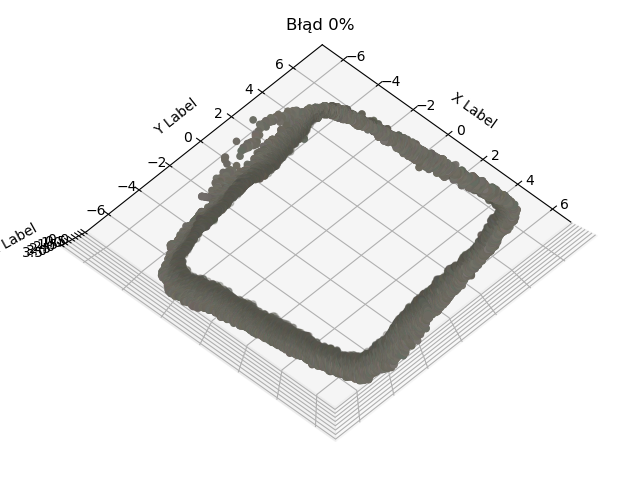
\includegraphics[scale=0.4]{blad_0.png}
  \caption{Widok kwadratowego pudełka z góry, dla 0\% błędu pomiarowego.}   
  \label{fig:zerobledu}
\end{figure}
Na rysunku ~\ref{fig:zerobledu} ukazane zostało pudełko z poprawnie zmierzoną odległością od środka tacki. Można zauważyć, że ma ono prostokątny kształt na płaszczyźnie XY. Środek modelu usytuowany jest w punkcie o współrzędnych (0,0). 
\begin{figure}[H]
  \centering
  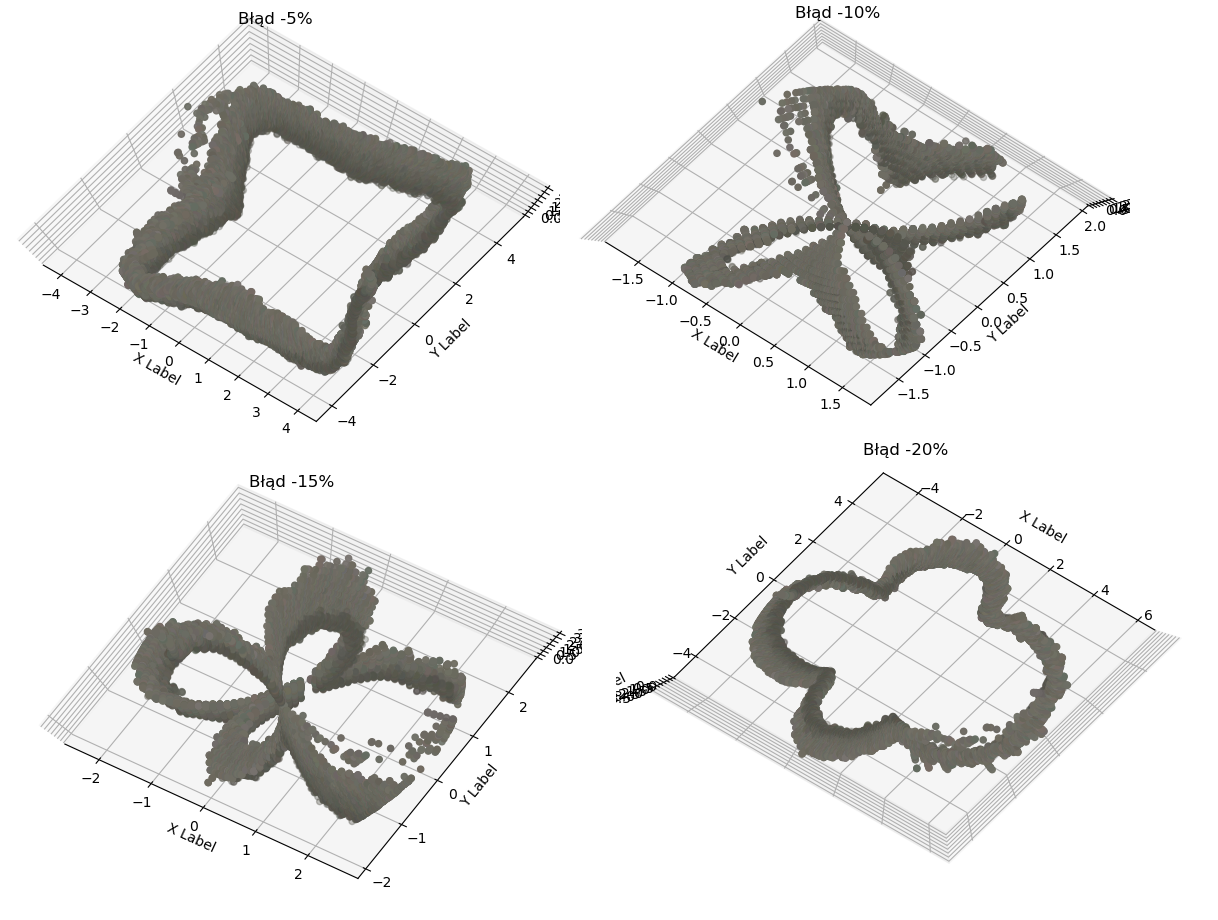
\includegraphics[scale=0.4]{bledyujemne.png}
  \caption{Porównanie wpływu ujemnego błędu pomiarowego na wygląd chmury punktów dla -5\%,-10\%,-15\%,-20\%.}   
  \label{fig:ujemnebledy}
\end{figure}
Na rysunku ~\ref{fig:ujemnebledy} dokonano porównania wpływu ujemnego błędu pomiarowego na ostateczny wynik chmury punktów. Dla błędu równego -5\%, czyli 47.5 cm zaczynają pojawiać się zniekształcenia. Dla -10\% oraz dla -15\% kształt obwodu chmury punktów zaczyna przypominać krzywą motylkową. Dla błędu -20\% nastąpiło przejście punktów na drugą stronę osi,a ich znak uległ zmianie.
\begin{figure}[H]
  \centering
  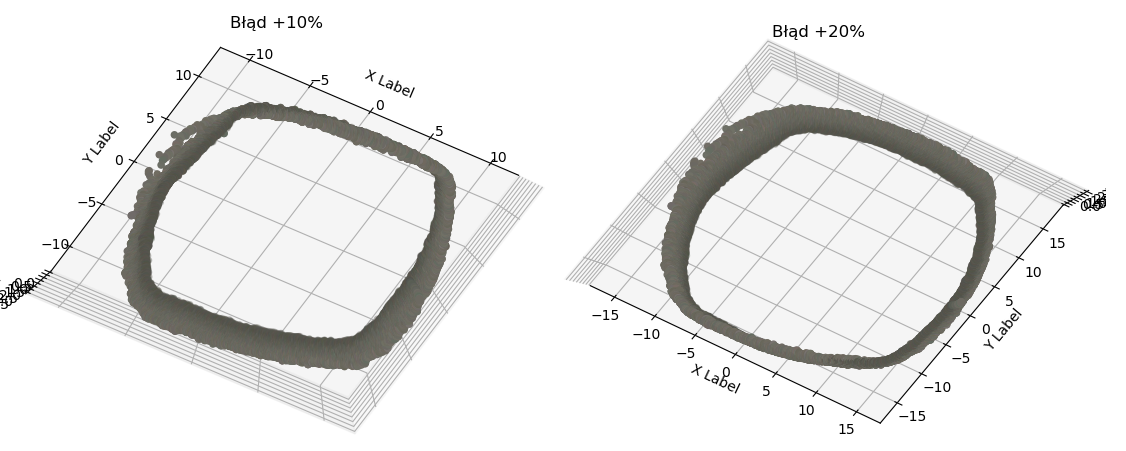
\includegraphics[scale=0.4]{bledydodatnie.png}
  \caption{Porównanie wpływu dodatniego błędu pomiarowego na wygląd chmury punktów dla +10\%,+20\%.}   
  \label{fig:dodatniebledy}
\end{figure}
Rysunek ~\ref{fig:dodatniebledy} przedstawia zmianę kształtu punktów przy dodatnim błędzie pomiarowym. Dla +10\% oraz +20\% następuje zaokrąglenie rogów. Wraz ze zwiększaniem błędu, kształt obrysu punktów zaczyna coraz bardziej przypominać okrąg.

Na powyższym porównaniu można zaobserwować jak duży wpływ na ostateczny wygląd modelu ma błędne zmierzenie odległości. Jeśli stosunek błędu do rzeczywistej odległości jest większy od 1, wtedy kształt modelu przybiera formę okręgu. Jeśli zaś jest mniejszy od 1, obwód modelu zaczyna być wklęsły. Przyczyną takiego zachowania algorytmu jest wzór wykorzystywany do przejścia ze współrzędnych obiektu do współrzędnych kamery. 
\begin{equation}
    \begin{aligned}
            & X_{\beta}=cos(\beta)(R-D_{\beta})  \\
            & Y_{\beta}=sin(\beta)(R-D_{\beta})  \\
    \end{aligned}
\end{equation}

$X_{\beta},Y_{\beta}$ są współrzędnymi punktu dla danego kąta $\beta$. R jest odległością od środka tacki. $D_{\beta}$ jest odległością danego punktu od kamery.

Z powyższego wzoru można wywnioskować, że gdy stosunek błędnie zmierzonej odległości od środka jest o wiele większy od rzeczywistej odległości, równania można zapisać następująco.
\begin{equation}
    \begin{aligned}
            &\frac{R_{b}}{D_{\beta}}>>\frac{R}{D_{\beta}} \implies\\
            & X_{\beta}=cos(\beta)R_{\delta}  \\
            & Y_{\beta}=sin(\beta)R_{\delta}  \\

    \end{aligned}
\end{equation}
$R_{b}$ jest błędnie zmierzoną odległością od środka tacki. $R_{\delta}$ jest promieniem zastępczym.

W powyższym wzorze widać, że im błędny pomiar jest większy od rzeczywistego pomiaru, tym bardziej współrzędne zaczynają przypominać punkty na okręgu. Co za tym idzie, uzyskany w rezultacie model obiektu będzie bardziej przypominał cylinder.

Z kolei, przy ujemnym błędzie pomiarowym, dla $R_{b}<<R$, promień $R-D_{\beta}$ może przybierać ujemne wartości. Dla błędu równego -15\% dostrzegalna jest zmiana wartości promienia z dodatniej na ujemną. 

Kolejnym krokiem jest wyznaczenie rzeczywistej wysokości obiektu na podstawie wykresu ~\ref{fig:wysokoscOdleglosc}. Wyznaczony empirycznie wzór pozwala na wyliczenie wysokości obiektu, znając odległość od niego oraz jego wymiary w pikselach. Znając wysokość obiektu jest możliwe ustalenie jaka powinna być gęstość punktów wzdłuż osi Z. Dzięki takiemu podejściu wymiary obiektu zostaną wiernie odwzorowane, a co za tym idzie, będzie można sprawdzić prawdziwe charakterystyki modelu. Mając informacje o rzeczywistych wymiarach, można ustalić objętość danego obiektu oraz jego powierzchnię w $m^2$.

Mając poprawnie wyznaczoną odległość od obiektu można przejść do wyznaczenia chmury punktów korzystając z równania ~\ref{equ:chmuraPunktow}. 

Do otrzymanej chmury punktów należy również dodać kolory poszczególnych pikseli uzyskane na podstawie obrazu RGB. Na potrzeby użytej metody zapisu trójwymiarowych modeli, piksele muszą zostać przeskalowane z wartości <0,255> do wartości z zakresu <0,1> dla każdego z trzech kolorów, czerwonego, zielonego oraz niebieskiego.
\subsection{Normalizacja punktów}
Istotnym aspektem działania algorytmu jest normalizacja punktów. Jest to proces mający na celu eliminację przekłamanych punktów, które mogą negatywnie wpływać na ostateczny wygląd modelu. Składa się on z kilku faz.
\newline \indent Pierwszym krokiem tej metody jest wyznaczenie średniej odległości wszystkich punktów od środka obiektu. Jest ona wyznaczana na podstawie poniższego wzoru.
\begin{equation}
    \begin{aligned}
            &D_{mean}=\frac{\sum_{n=0}^{N} \sqrt{p_{nx}^2+p_{ny}^2}}{N}  
    \end{aligned}
\end{equation}
$p_{nx},p_{ny}$ są współrzędnymi n-tego punktu P. N jest łączną ilością punktów w zbiorze. D jest średnią odległością punktu od środka układu. Warto zauważyć, że we wzorze nie występuję współrzędna Z n-tego punktu. Powodem tego jest fakt, iż punkty są równomiernie rozłożone wzdłuż osi Z. Liczenie odległości wzdłuż tej osi nie wpłynęło by na poprawienie dokładności wyznaczania odpowiednich punktów. Można więc ten etap pominąć i wykorzystać jedynie dwie pierwsze współrzędne punktu do wyznaczenia jego pozycji względem środka.
\newline \indent Dla każdego punktu ze zbioru sprawdzana jest odległość od środka. Jeśli jest ona większa, niż $p\% \cdot D_{mean}$, gdzie $p\%$ oznacza graniczny współczynnik odległości od środka, to punkt zostaje oznaczony odpowiednią flagą. Flaga umożliwia w późniejszym etapie rozpoznanie przekłamanego punktu oraz dodanie go do zbioru interpolacyjnego.
\subsection{Interpolacja punktów}
Po tym jak wszystkie przekłamane punkty zostały odpowiednio oznaczone można przejść do ich interpolacji. Wykorzystując technikę interpolacji można wyznaczyć współrzędne tych punktów, których wartości początkowo były błędne. Podczas badań otrzymanych rezultatów interpolacji, został wybrany najlepszy algorytm. Spośród interpolacji liniowej,sześciennej oraz najbliższych sąsiadów wybrana została metoda sześcienna. Daje ona najlepsze rezultaty spośród wszystkich wypróbowanych metod. Punkty zostały przekształcone za pomocą wzoru ~\ref{equ:wielomianowaEqu}. Wynikiem takiej operacji jest nowa chmura punktów, która nie zawiera już przekłamanych wartości. Dzięki temu możliwe będzie dokładne utworzenie siatki triangulacyjnej na modelu. Korzystając z danej metody interpolacji uzyskane wartości mają bardziej naturalny rozkład. W przypadku jej liniowej odmiany, współrzędne punktów rosły liniowo. Sprawiało to wrażenie, że punkty na obiekcie były ułożone błędnie. Po zmianie na interpolację wielomianem trzeciego stopnia, ten problem jest niezauważalny.  
\section{Porównanie metod rekonstrukcji powierzchni}
W poniższej sekcji przedstawione zostały wyniki implementacji dwóch metod rekonstrukcji powierzchni. Dokonano porównania dokładności odwzorowania powierzchni jak również ich szczegółowości. W algorytmie BPA porównano wpływ promienia kuli na ostateczny wygląd modelu oraz czas trwania algorytmu. Dla triangulacji Delaunay'a zostanie przedstawiona szczegółowa implementacja oraz użyte metody optymalizacji. Ukazany zostanie również wpływ ilości punktów na czas trwania triangulacji.

\subsection{Algorytm BPA}
Dla porównania został zaimplementowany algorytm BPA. Jego użycie jest możliwe dzięki wykorzystaniu biblioteki Open3D. Pakiet umożliwia dokonywanie wielu operacji na chmurach punktów. Dostępne są w nim rekonstrukcje Poissona, wyznaczanie wektorów normalnych oraz dane testowe do przeprowadzania badań dokładności implementowanych algorytmów. Na potrzeby wdrożenia danej metody wykorzystana zostanie funkcja umożliwiająca stworzenie meshu przy wykorzystaniu algorytmu BPA. Implementacja algorytmu składa się z kilku kroków które zostały omówione poniżej.
\subsubsection{Estymacja normalnych}
Główną ideą algorytmu jest toczenie kuli po chmurze punktów. W przypadku kiedy gęstość 3 dotkniętych punktów jest większa od średniej gęstości to utworzony w ten sposób trójkąt będzie mniejszy. W przypadku, gdy lokalna gęstość jest jednak mniejsza niż średnia, kula może dotknąć punktu, który jest ukryty. Znajduje się on wtedy pod górną warstwą i w celu dokładnego odwzorowania powierzchni, tak utworzony trójkąt powinien zostać odrzucony \cite{mittleman1999ball}. Dana sytuacja została opisana na rysunku \ref{fig:bpaWrongTria}.
\begin{figure}[H]
  \centering
  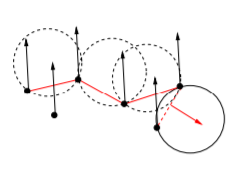
\includegraphics[scale=0.8]{bpa_wrong.PNG}
  \caption{Dotknięcie przez kule punktu pod powierzchnią \cite{mittleman1999ball}.}   
  \label{fig:bpaWrongTria}
\end{figure}

W celu wykrycia poprawnie skonstruowanego trójkąta używane są normalne. W tym celu należy obliczyć wektory normalne do powierzchni danego trójkąta oraz do średnie wektory normalne do powierzchni blisko danego trójkąta. 
\begin{equation}
    \begin{aligned}
            &N_{tri}=\vec{AB} \times \vec{AC}\\
            &N_{mean}=\frac{\sum_{i=1}^{N} \vec{A_{i}B_{i}} \times \vec{A_{i}C_{i}}}{N}\\
            & |N_{tri}||N_{mean}|cos(\theta)=N_{tri} \cdot N_{mean}\\
            &\theta=arccos(\frac{N_{tri} \cdot N_{mean}}{|N_{tri}||N_{mean}|})

    \end{aligned}
\end{equation}
$N_{tri}$ jest wektorem normalnym do powierzchni trójkąta. $N_{tri}$ jest wektorem normalnym do powierzchni wokół danego trójkąta interpolacyjnego. $\theta$ jest kątem pomiędzy wektorem normalnym do trójkąta, a powierzchnią wokół niego. 
\newline \indent Trójkąt interpolacyjny należy odrzucić, gdy iloczyn skalarny jego wektora normalnego oraz normalnej do powierzchni jest ujemny. Oznacza to, że kąt $\theta$ pomiędzy nimi będzie większy od $\frac{\pi}{2}$. Dla wartości powyżej 90 stopni trójkąt będzie skierowany przeciwnie do powierzchni i należy go odrzucić. Do wyznaczenia wektorów normalnych do chmury punktów użyta została funkcja dostępna w bibliotece open3D. Znajduje ona punkty w okolicy danego punktu i przecinając je prostą tworzy wektor normalny. Następnie wektory normalne do punktu są uśredniane i wyznaczane za pomocą analizy kowariancji.
\subsubsection{Wyznaczenie średniej odległości punktów}
Kolejnym krokiem potrzebnym do poprawnego funkcjonowania algorytmu BPA jest odpowiedni dobór promienia kuli R. Jest to bardzo istotny parametr algorytmu. Odpowiedni jego dobór sprawi, że wyjściowy model trójwymiarowy obiektu będzie szczegółowy i będzie zawierał mało luk. Jednakże wraz ze wzrostem długości promienia rośnie również czas obliczeniowy programu. Promień powinien być więc dobierany z uwzględnieniem obu tych aspektów. W celu jego najlepszego doboru należy wyznaczyć średnią odległość punktów od siebie. Znając tę odległość, będzie można odpowiednio dobrać długość R, by kula nie wpadała w przestrzenie pomiędzy punktami. Za obliczenie średnich odległości odpowiada funkcja z biblioteki open3D. Dla każdego punktu w chmurze wyznacza jest odległość od najbliższego sąsiada. Z tak powstałego wektora odległości można wyznaczyć średnią korzystając z biblioteki Numpy w celu optymalizacji czasu obliczeniowego. Następnie, traktując średnią odległość pomiędzy obiektami jako punkt wyjściowy, można empirycznie dobrać odpowiednią wartość promienia kuli R. W tabeli \ref{tab:bpaRInfluence} został przedstawiony wpływ wielkości promienia R na czas trwania obliczeń oraz ilość trójkątów.
\begin{table}[H] 
\begin{center}
\caption{\label{tab:bpaRInfluence}Czas trwania triangulacji metodą BPA w zależności od długości promienia R dla średniej odległości między punktami równej D_{mean}=0.047.}
\centerline{
\begin{tabular}{ |c|c|c|c| }
 \hline
 { Długość promienia} & { $\frac{R}{D_{mean}}$ }&{ Czas trwania}& { Liczba trójkątów}\\ 
  \hline
   {\small 0.047 } & {\small 1} & {\small 0.51 s}& {\small 42819}  \\  
  \hline 
     {\small 0.09 } & {\small 2} & {\small 1.44 s}& {\small 44025}  \\  
  \hline 
   {\small 0.14 } & {\small 3} & {\small 7.5 s}& {\small 32474}  \\  
  \hline 
     {\small 0.19 } & {\small 4} & {\small 29.8 s}& {\small 24936}  \\  
  \hline 
       {\small 0.23 } & {\small 5} & {\small 93 s}& {\small 21496}  \\  
  \hline 
         {\small 0.28 } & {\small 6} & {\small 215 s}& {\small 18641}  \\  
  \hline 
           {\small 0.33 } & {\small 7} & {\small 430 s}& {\small 16348}  \\  
  \hline 
             {\small 0.38 } & {\small 8} & {\small  737s}& {\small 14457}  \\  
  \hline 

\end{tabular}
}
\end{center}
\end{table}
W powyższej tabeli przedstawiony został wpływ wielkości promienia na czas obliczeń oraz liczbę trójkątów. Z danych zebranych podczas testów można wysnuć wniosek, iż wraz ze wzrostem długości promienia kuli, rośnie czas trwania algorytmu. Maleje przy tym ilość utworzonych trójkątów. Podstawą takiego zachowania jest fakt, iż przy większym promieniu kula dotyka mniejszej ilości punktów, tym samym tworząc mniej trójkątów. Jednocześnie czas trwania algorytmu rośnie, ponieważ badanie sąsiedztwa punktów zajmuje więcej czasu. Przy większym promieniu kuli, poszukiwana jest liczba sąsiadów danego punktu w większym otoczeniu. To znacząco wpływa na złożoność obliczeniową.
\newline \indent Po wyznaczeniu normalnych oraz dobraniu promienia kuli ostatnim krokiem jest utworzenie triangulacji BPA. Wykorzystując funkcję z biblioteki open3D można przeprowadzić algorytm toczącej się kuli i uzyskać ściany trójkątów triangulacyjnych. Funkcja dostępna w bibliotece jest udoskonaleniem początkowej metody zaproponowanej przez Bernardini w 1999 roku. Wprowadza ona możliwość równoległego przeprowadzania obliczeń w celu ich szybszego wykonywania \cite{digne2014analysis}. By z większą prędkością odnajdywać sąsiadujące punkty użyto również drzewa ósemkowego. Jest to struktura danych umożliwiająca podzielenie przestrzeni na mniejsze części, a następnie utworzenie drzewa sąsiedztw. Znając strukturę drzewa, można je przeszukiwać w bardzo łatwy sposób, by odnaleźć odpowiednich sąsiadów punktu. Tworzenie tej struktury ma charakter rekurencyjny. Początkowo generowany jest sześcian otaczający wszystkie punkty, następnie jest on dzielony na 4 sześciany. Każdy kolejny na kolejne 4 rekurencyjnie. Podział trwa do momentu, kiedy wewnątrz sześcianu znajduje się nie więcej niż 8 punktów. Każdy korzeń w drzewie ma 8 gałęzi. Współrzędne każdego punktu w drzewie można zapisać binarnie. Znając pozycję danego punktu w drzewie, korzystając ze wzoru oraz przesunięć binarnych można odnaleźć jego sąsiadów. Dzięki tym operacjom przeprowadzony zostanie algorytm BPA znacznie szybciej, niż jego początkowa implementacja z 1999 roku. W ten sposób powstały model może wciąż zawierać luki, wynikające z nierównomiernej gęstości punktów. Na koniec otrzymane trójkąty triangulacyjne można wyeksportować do pliku obsługiwanego przez program Blender. W tym programie można dodać ręcznie płaszczyzny by zakryć luki powstałe w skutek przeprowadzenia algorytmu BPA. 




\subsection{Triangulacja Delaunay'a}
W celu implementacji trójwymiarowej metody triangulacji Delaunay'a zastosowano algorytm Bowyer-Watson \cite{rebay1993efficient}. Przedstawia on sposób na dołączanie dodatkowych punktów do triangulacji oraz sposób na jej utworzenie. Przy początkowej implementacji algorytmu, czas obliczeń był zbyt długi. Ilość punktów występująca przy triangulacji rzeczywistych danych pomiarowych sięga około 20000. Potrzebna była metoda szybszego obliczania triangulacji oraz generacji meshu. Dokonano wielu kluczowych optymalizacji mających na celu minimalizację czasu trwania programu. Początkowe czasy trwania obliczeń zostały przedstawione w tabeli \ref{tab:firstVersionPython}. 
\begin{table}[H]
\begin{center}
\caption{\label{tab:firstVersionPython}Czas trwania triangulacji przed optymalizacją.}
\centerline{
\begin{tabular}{ |c|c| }
 \hline
 { Liczba punktów} & { Czas}\\ 
  \hline
   {\small 1000 pkt} & {\small 10.85 s}   \\  
  \hline 
     {\small 5000 pkt} & {\small 246 s}   \\  
  \hline
   {\small  10000 pkt} & {\small 915 s}   \\  
  \hline
\end{tabular}
}
\end{center}
\end{table}
W powyższej tabeli można dostrzec, iż czas triangulacji przekracza początkowe założenia. Maksymalna zbadana ilość punktów testowych wynosi 10000. Czas triangulacji takiej ilości punktów powinien być znacząco niższy. Poprawiono, więc metody użyte w algorytmie, by zwiększyć jego wydajność. Głównym aspektem algorytmu, który potrzebował najwięcej czasu obliczeniowego jest wyznaczenie przynależności punktu do sfery opisanej na czworościanie. Dokonano porównania dwóch metod wyznaczania środka sfery opisanej na czworościanie.
\subsubsection{Wykorzystanie iloczynu skalarnego oraz wektorowego}
Pierwsza metoda oparta jest o kombinację iloczynu wektorowego oraz skalarnego w celu uzyskania współrzędnych środka okręgu \cite{CircumTetraMath}. Wykorzystując podstawowe przekształcenia geometryczne, na podstawie współrzędnych wierzchołków możliwe jest określenie współrzędnych barycentrum. Równanie przedstawiające wzór na środek sfery opisanej na ostrosłupie zostało przedstawione poniżej.
\begin{equation}
    \begin{aligned}
            &u_{i}=v_{i}-v_{0} , i=1,2,3\\
            &p=O-v_{0}\\
            &R^2=\lVert p^2 \rVert=\lVert u_{1}-p \rVert^2=\lVert u_{2}-p \rVert^2=\lVert u_{3}-p \rVert^2\\
            &O=v_{0}+\frac{l_{01}^2(u_{2}\times u_{3})+l_{02}^2(u_{3}\times u_{1})+l_{03}^2(u_{1}\times u_{2})}{2u_{1}\cdot (u_{2}\times u_{3})}
    \end{aligned}
\end{equation}
$v_{0} \dots v_{3}$ są wierzchołkami czworościanu. $U_{i}$ jest wektorem przejścia z wierzchołka $v_{0} do v_{i}$. O jest środkiem sfery opisanej na czworościanie. p jest wektorem przejścia z wierzchołka $v_{0}$ do środka sfery opisanej na czworościanie O. R jest promieniem sfery. $l_{0i}$ jest długością krawędzi łączącej wierzchołek $v_{0}$ oraz $v_{i}$.
\newline \indent W powyższych wzorach znajdują się 4 iloczyny wektorowe oraz jeden iloczyn skalarny. Wszystkie te operacje są bardzo kosztowne obliczeniowo. W tabeli \ref{tab:oldCircumSphere} przedstawione zostały czasy triangulacji w zależności od ilości punktów. Pomiary są znacznie lepsze niż na początku, lecz wymagana jest dalsza ich optymalizacja.
\begin{table}[H]
\begin{center}
\caption{\label{tab:oldCircumSphere}Czasy triangulacji dla pierwszej metody wyznaczania przynależności punktu do sfery.}
\centerline{
\begin{tabular}{ |c|c| }
 \hline
 { Liczba punktów} & { Czas}\\ 
  \hline
   {\small 1000 pkt} & {\small 4.55 s}   \\  
  \hline 
     {\small 5000 pkt} & {\small 67 s}   \\  
  \hline
   {\small  10000 pkt} & {\small 194 s}   \\  
  \hline
  {\small  15000 pkt} & {\small 455 s}\\
  \hline
\end{tabular}
}
\end{center}
\end{table}
\subsubsection{Metoda wyznaczników macierzy}
Druga metoda określania współrzędnych środka sfery opisanej na czworościanie polega na obliczeniu wyznaczników \cite{CircumTetraWolf}. Z punktu widzenia złożoności obliczeniowej jest ona bardziej optymalna w porównaniu do pierwszej metody. Równania zawierające odpowiednie przekształcenia zostały przedstawione poniżej.
\begin{equation}
    \begin{aligned}
            &0=\begin{vmatrix}
                x^2+y^2+z^2 & x&y&z&1 \\
                x_{1}^2+y_{1}^2+z_{1}^2 & x_{1}&y_{1}&z_{1}&1 \\
                x_{2}^2+y_{2}^2+z_{2}^2 & x_{2}&y_{2}&z_{2}&1 \\
                x_{3}^2+y_{3}^2+z_{3}^2 & x_{3}&y_{3}&z_{3}&1 \\
                x_{4}^2+y_{4}^2+z_{4}^2 & x_{4}&y_{4}&z_{4}&1 \\
            \end{vmatrix}\\
            \text{Po przekształceniu wyznacznika}\\
            &a(x^2+y^2+z^2)-(D_{x}x+D_{y}y+D_{z}z)+c=0\\
            &a=\begin{vmatrix}
               x_{1}&y_{1}&z_{1}&1 \\
                x_{2}&y_{2}&z_{2}&1 \\
                x_{3}&y_{3}&z_{3}&1 \\
                x_{4}&y_{4}&z_{4}&1 \\
            \end{vmatrix}\\
            &D_{x}=\begin{vmatrix}
                x_{1}^2+y_{1}^2+z_{1}^2 &y_{1}&z_{1}&1 \\
                x_{2}^2+y_{2}^2+z_{2}^2 & y_{2}&z_{2}&1 \\
                x_{3}^2+y_{3}^2+z_{3}^2 &y_{3}&z_{3}&1 \\
                x_{4}^2+y_{4}^2+z_{4}^2 &y_{4}&z_{4}&1 \\
            \end{vmatrix}\\
            &D_{y}=-\begin{vmatrix}
                x_{1}^2+y_{1}^2+z_{1}^2 &x_{1}&z_{1}&1 \\
                x_{2}^2+y_{2}^2+z_{2}^2 &x_{2}&z_{2}&1 \\
                x_{3}^2+y_{3}^2+z_{3}^2 &x_{3}&z_{3}&1 \\
                x_{4}^2+y_{4}^2+z_{4}^2 &x_{4}&z_{4}&1 \\
            \end{vmatrix}\\
                &D_{y}=\begin{vmatrix}
                x_{1}^2+y_{1}^2+z_{1}^2 &x_{1}&y_{1}&1 \\
                x_{2}^2+y_{2}^2+z_{2}^2 &x_{2}&y_{2}&1 \\
                x_{3}^2+y_{3}^2+z_{3}^2 &x_{3}&y_{3}&1 \\
                x_{4}^2+y_{4}^2+z_{4}^2 &x_{4}&y_{4}&1 \\
            \end{vmatrix}\\
            &c=\begin{vmatrix}
                x_{1}^2+y_{1}^2+z_{1}^2 &x_{1}&y_{1}&z_{1} \\
                x_{2}^2+y_{2}^2+z_{2}^2 &x_{2}&y_{2}&z_{2} \\
                x_{3}^2+y_{3}^2+z_{3}^2 &x_{3}&y_{3}&z_{3} \\
                x_{4}^2+y_{4}^2+z_{4}^2 &x_{4}&y_{4}&z_{4} \\
            \end{vmatrix}\\
            \text{Po podstawieniu do równania opisującego sferę}\\
            &(x-x_{0})^2+(y-y_{0})^2+(z-z_{0})^2=r^2\\
            &a(x-\frac{D_{x}}{2a})^2+a(y-\frac{D_{y}}{2a})^2+a(z-\frac{D_{z}}{2a})^2-\frac{D_{x}^2+D_{y}^2+D_{z}^2}{4a}+c=0\\
            \text{Współrzędne środka sfery}\\
            &x_{0}=\frac{D_{x}}{2a}\\
            &y_{0}=\frac{D_{y}}{2a}\\
            &z_{0}=\frac{D_{z}}{2a}\\
            &r=\frac{\sqrt{D_{x}^2+D_{y}^2+D_{z}^2-4ac}}{2|a|}
    \end{aligned}
\end{equation}
$x_{i},y_{i},z_{i}$ są współrzędnymi i-tego wierzchołka czworościanu, dla i=1,2,3. $x_{0},y_{0},z_{0}$ są współrzędnymi środka sfery opisanej na czworościanie. R jest promieniem tej sfery.
\newline \indent Z powyższych równań wynika, że do obliczenia współrzędnych środka okręgu wystarczy określić 4 wyznaczniki macierzy. Jest to operacja o wiele szybsza niż liczenie iloczynów wektorowych i skalarnych. W celu większej optymalizacji promień sfery został obliczony jako odległość wierzchołka od środka okręgu. W porównaniu do obliczania kolejnych dwóch wyznaczników macierzy a oraz c, jest to szybsza operacja. Zestawienie czasu trwania algorytmów dla obu wymienionych metod zostało przedstawione w tabeli \ref{tab:bothMethodsCircumsphere}.
\begin{table}[H]
\begin{center}
\caption{\label{tab:bothMethodsCircumsphere}Czasy triangulacji dla pierwszej oraz drugiej metody wyznaczania przynależności punktu do sfery.}
\centerline{
\begin{tabular}{ |c|c|c| }
 \hline
 { Liczba punktów} & { Czas metody iloczynowej}& { Czas metody wyznaczników}\\ 
  \hline
   {\small 1000 pkt} & {\small 4.55 s} & {\small 2.97 s}  \\  
  \hline 
     {\small 5000 pkt} & {\small 67 s}& {\small 40 s}   \\  
  \hline
   {\small  10000 pkt} & {\small 194 s}& {\small 179 s}   \\  
  \hline
 {\small  15000 pkt} & {\small 455 s}& {\small 448 s}   \\  
  \hline
\end{tabular}
}
\end{center}
\end{table}
Dane przedstawione w powyższej tabeli świadczą o wyższości drugiej metody nad pierwszą. Oba algorytmy zawierają przekształcenia macierzowe. W metodzie iloczynowej zawarte są 4 iloczyny wektorowe oraz jeden iloczyn skalarny. W metodzie wyznacznikowej obliczane są 4 wyznaczniki macierzy. Widać, iż w drugim przypadku obliczenia okazały się być mniej złożone. Średni spadek czasu trwania programu wynosił 30\% względem pierwszej metody. Z powyższej tabeli wynika również, że wraz ze wzrostem ilości punktów maleje różnica pomiędzy tymi dwoma metodami. Wynika to ze stałej różnicy kosztu obliczeniowego dla pierwszej oraz drugiej metody. Wiele czynników wpływa na wydłużenie czasu trwania algorytmu. Podstawowym parametrem jest ilość punktów. Jako, że różnica między dwoma metodami jest stała, a cały algorytm jest zależny od objętości chmury punktów, to różnica pomiędzy nimi spada wraz ze wzrostem ilości punktów.
\newline \indent Kolejną znaczącą optymalizacją dokonaną w programie jest przejście z języka python do cython. Oba te języki programowania posiadają bardzo podobną strukturę, jednakże znacząco różnią się one sposobem wykonywania programu. Python jest językiem interpretowanym. Program punkt po punkcie uruchamia każdą instrukcję i wykonuje ją w locie. Dzięki tej możliwości, nawet jeśli w późniejszym etapie programu jest błąd, zostanie on wykryty dopiero w momencie wykonania instrukcji. Z kolei cython jest językiem kompilowanym. Każdy plik wchodzący w skład programu jest kompilowany do języka C. Szereg instrukcji dla programu jest odgórnie wyznaczony, a wszystkie operacje mogą zostać wstępnie przekształcone do języka maszynowego. Dzięki takiej operacji wydajność programu znacznie się zwiększyła. W celu sprawdzenia wzrostu wydajności dzięki zastosowaniu języka cython dokonano porównania. Zaimplementowano dwa jednakowe algorytmy, jeden napisany w języku python, drugi zaś w cython. Wyniki pomiarów znajdują się w tabeli \ref{tab:cythonVsPython}.
\begin{table}[H]
\begin{center}
\caption{\label{tab:cythonVsPython}Porównanie czasu trwania algorytmu dla cython oraz python.}
\centerline{
\begin{tabular}{ |c|c|c| }
 \hline
 { Liczba punktów} & { Czas cython}& { Czas python}\\ 
  \hline
   {\small 1000 pkt} & {\small 2.97 s} & {\small 6 s}  \\  
  \hline 
     {\small 5000 pkt} & {\small 40 s}& {\small 132 s}   \\  
  \hline
   {\small  10000 pkt} & {\small 179 s}& {\small  543 s}   \\  
  \hline
 {\small  15000 pkt} & {\small 448 s}& {\small  1285 s}   \\  
  \hline
\end{tabular}
}
\end{center}
\end{table}

\begin{figure}[H]
  \centering
  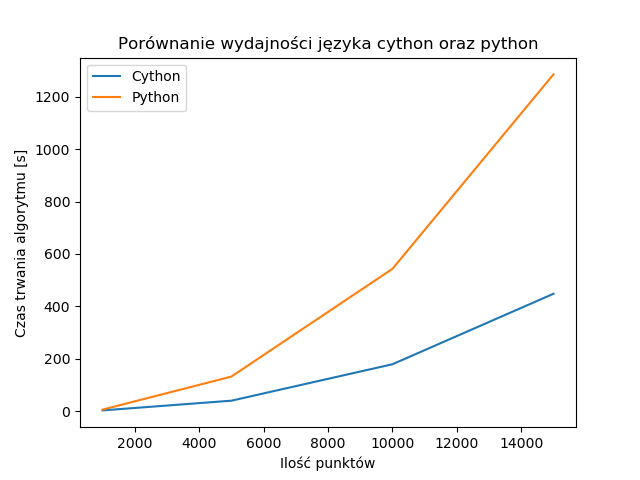
\includegraphics[scale=0.6]{pythonvscython.png}
  \caption{Porównanie czasu algorytmu dla cython oraz python.}   
  \label{fig:pytcytpic}
\end{figure}

Na wykresie \ref{fig:pytcytpic} oraz w tabeli \ref{tab:cythonVsPython} można zauważyć, że wstępna kompilacja kodu nie tylko wpłynęła procentowo na wydajność algorytmu. Sprawiła ona, iż tempo wzrostu złożoności obliczeniowej w zależności od ilości punktów również się zmniejszyło. Dzięki temu możliwe jest wykonanie triangulacji jeszcze większej ilości punktów. Zmniejszenie tempa wzrostu ma związek z optymalizacją pętli iteracyjnych w języku cython. Wraz ze wzrostem ilości punktów poddanych triangulacji, rośnie również ilość iteracji pętli. W języku python pętle wykonywane są wolniej niż w cython, dlatego też przyrost czasu obliczeniowego jest znacznie bardziej dostrzegalny.

Następnym elementem który wpłynął pozytywnie na optymalizację czasu działania programu jest zmiana biblioteki. Dotychczas do obliczania wyznacznika macierzy używana była funkcja z biblioteki NumPy. Jest to biblioteka typu open-source. Dostęp do niej jest darmowy, a aktualizować ją może każdy kto zostanie zaakceptowany przez społeczność. Dzięki pracy dużej liczby ludzi kod jest zoptymalizowany oraz uniwersalny. Funkcje dostępne w NumPy mają bardzo dużą wydajność pod względem pamięci i zasobów obliczeniowych. Biblioteka zawiera wiele różnych modułów począwszy od algebry liniowej, po równania różniczkowe oraz obliczenia na liczbach zespolonych. Z testów przeprowadzonych na programie do triangulacji wynika, że do obliczeń macierzowych najlepiej jednak się biblioteka SciPy. Ona też jest zbiorem programów typu open-source. Korzysta ona po części z NumPy jako struktury do przechowywania danych obliczeniowych. Obie biblioteki zawierają podobne funkcje, lecz do zastosowań projektowych wybrana została ta druga. Porównanie pracy programu, przy zastosowaniu funkcji z biblioteki NumPy oraz SciPy do obliczeń macierzowych zostało przedstawione w tabeli \ref{tab:numpyVsScipy}.
\begin{table}[H]
\begin{center}
\caption{\label{tab:numpyVsScipy}Porównanie czasu trwania algorytmu przy obliczaniu macierzy przez NumPy oraz SciPy.}
\centerline{
\begin{tabular}{ |c|c|c| }
 \hline
 { Liczba punktów} & { Czas SciPy}& { Czas NumPy}\\ 
  \hline
   {\small 1000 pkt} & {\small 2.97 s} & {\small 2.48 s}  \\  
  \hline 
     {\small 5000 pkt} & {\small 40 s}& {\small 36 s}   \\  
  \hline
   {\small  10000 pkt} & {\small 179 s}& {\small  231 s}   \\  
  \hline
 {\small  15000 pkt} & {\small 448 s}& {\small  486 s}   \\  
  \hline
\end{tabular}
}
\end{center}
\end{table}
W powyższej tabeli został przedstawiony wpływ użycia różnych bibliotek na ostateczny czas trwania algorytmu triangulacji Delaunay'a. Dla mniejszej ilości punktów, biblioteka NumPy jest wydajniejsza. Jednak przy wzroście punktów, biblioteka SciPy osiągnęła lepsze wyniki, dlatego została wybrana jako docelowa metoda przeprowadzania obliczeń macierzowych.  

Kolejnym aspektem algorytmu wymagającym znacznej mocy obliczeniowej jest badanie styczności czworościanów. W algorytmie, z każdej ściany ostrosłupa niestykającej się z inną ścianą jest budowany jest dodatkowy czworościan. W jego skład wchodzą trzy wierzchołki początkowej ściany oraz dodatkowy punkt triangulacyjny. Należy, więc znaleźć te ściany algorytmu, które nie stykają się z pozostałymi. Jest to zadanie wymagające dwóch pętli iteracyjnych i wykonywane jest dla każdego dodatkowego punktu. W przypadku autorskiego programu, zostało zastosowane kryterium przynależności zbiorów. Tablica ścian została utworzona poprzez kombinację 4 różnych wierzchołków. Dla każdego z pozostałych czworościanów sprawdzane jest czy którekolwiek z trzech wierzchołków znajdują się w zbiorze ścian początkowego ostrosłupa. Jeśli tak, to ściana ta jest dodawana do zbioru zajętych ścian i proces jest kontynuowany do momentu wyczerpania pozostałych ostrosłupów lub ścian. Zadanie to nie jest trywialne z punktu widzenia struktury danych. Matematyczne podstawy jego funkcjonowania nie są złożone, jednakże opis programowy tak. Wymagana jest struktura, która umożliwia przechowywanie nieuporządkowanej sieci wierzchołków. Dzieje się tak ze względu na to, że punkty mogą tworzyć ścianę w różnej kolejności, więc porządek ich występowania w danej ścianie może być różny dla dwóch osobnych ostrosłupów. Zostały sprawdzone dwie metody odnajdywania sąsiadujących ścian.
\newline \indent Pierwsza metoda zakładała iterację przez wszystkie wierzchołki początkowego oraz aktualnego czworościanu. Dzięki temu można było sprawdzić ile z nich występuje w obu tych zbiorach. To zadanie wymagało dużo czasu obliczeniowego, ponieważ korzystało z trzech pętli iteracyjnych. Pierwsza odpowiadała za wybór sąsiedniego ostrosłupa, druga za wybór ściany do sprawdzenia w aktualnym czworościanie, a trzecia za wybór ściany w drugim ostrosłupie.
\newline \indent Drugą metodą, która była możliwa dzięki zastosowaniu języka python były operacje na zbiorach. Struktura danych set() umożliwia przechowywanie nieuporządkowanych zbiorów danych i dokonywanie na nich operacji. Na potrzeby algorytmu triangulacyjnego zastosowano iloczyn dwóch zbiorów.
\begin{equation}
    \begin{aligned}
    &V_{a}={v_{a1},v_{a2},v_{a3},v_{a4}}\\
    &V_{b}={v_{b1},v_{b2},v_{b3},v_{b4}}\\
    &S_{a}=\binom{V_{a}}{3}\\
    &S_{b}=\binom{V_{b}}{3}\\
    &W=V_{a} \cap V_{b}\\
    &S_{bi} 	\subset S_{a} \Leftrightarrow |W|=3\\
    &S_{f}=S_{a}/S_{bi}
    \end{aligned}
\end{equation}
$V_{a},V_{b}$ są zbiorami wierzchołków ostrosłupa A oraz B. $S_{a},S_{a}$ jest zbiorem ścian ostrosłupa A oraz B. W jest zbiorem wspólnych wierzchołków ostrosłupów. $S_{f}$ jest zbiorem ścian niestykających się z innym ostrosłupem.
\newline \indent Z powyższych równań widać, że jeśli moc zbioru będącego iloczynem zbiorów wierzchołków ostrosłupów będzie równa 3, to obie te figury będą posiadały wspólną ścianę. Należy ją wtedy dodać do zbioru współdzielonych ścian. Operacja zostanie powtórzona dla wszystkich pozostałych ostrosłupów. Ze ścian wolnych które pozostaną, zostaną zbudowane nowe ostrosłupy.
\newline \indent Na sam koniec, ze zbioru ostrosłupów triangulacyjnych należy usunąć te, które współdzielą wierzchołki z początkowym super-ostrosłupem.
\newline \indent Powyższe operacje przedstawiają algorytm triangulacji Delaunay'a, dzięki któremu uzyskiwane są ostrosłupy. Do generacji meshu potrzebna jest jeszcze dodatkowa rzecz. Mianowicie, muszą zostać utworzone poszczególne ściany tych ostrosłupów. Są one generowane poprzez kombinację wierzchołków ostrosłupa. Następnie, współrzędne wierzchołków muszą zostać przekształcone na odpowiadające im indeksy w zbiorze punktów. W celu optymalizacji algorytmu każdy punkt posiada czwartą współrzędną. Jest nią indeks na którym znajduje się punkt w ogólnym zbiorze punktów. Umożliwia to w końcowym etapie szybkie przekształcenie ścian bryły do postaci indeksów.
\newline \indent Ostatnim etapem programu jest zapis utworzonego w ten sposób meshu do pliku. Wykonywane jest to za pomocą biblioteki trimesh. Jako parametr podawany jest tam zbiór ścian ostrosłupa. Kolejnymi parametrami są kolory wierzchołków oraz ich współrzędne. Tak wygenerowany plik może zostać wyeksportowany i otwarty w programie Blender. Można tam dokonywać różnych operacji na danym modelu, poddawać go przekształceniom w przestrzeni oraz go skalować.
